\section{Coresets and Sensitivity Sampling}

In this work, we are using the method of coresets
(see for example~\cite{munteanu-coresets-introduction})
to approach the problem of data reduction for the probit model.
The idea behind coresets is, that when given a
dataset $\mathcal{D}$, we are interested in selecting
only a small subset of observations
$\mathcal{C} \subseteq \mathcal{D}$, such that the objective
function evaluated on the (possible reweighted) subset $\mathcal{C}$
does not differ too much
from the objective function evaluated on the original dataset $\mathcal{D}$.

This approach will allow us to estimate the model parameters
efficiently on the ideally much smaller set $\mathcal{C}$,
when a full optimization on $\mathcal{D}$ could already
be infeasible for big datasets.
We are thus following the paradigm of \textit{sketch-and-solve},
i.e. first reducing the size of the original dataset and then solving
the optimization problem on the reduced dataset.

In order to work out a formal definition of when we call a subset
$\mathcal{C} \subseteq \mathcal{D}$ a coreset in the context of
probit regression, we first have to slightly extend the
concept of the model matrix, as we will need it for the coreset
definition.

\begin{definition}[Scaled model matrix]
    Let $\mathcal{D}=\{(x_i, y_i)\}_{i=1}^n$ be a $d$-dimensional dataset.
    Let $z_i = (2y_i - 1)x_i$ for all i in $[n]$.
    Then we call the matrix $Z \in \mathbb{R}^{n \times d}$, where the
    $i$-th row consists of the vector $z_i$ for all $i \in [n]$,
    the scaled model matrix of $\mathcal{D}$.
\end{definition}

This definition of the scaled model matrix is nothing particularly new,
it just formalizes the concept of factoring the labels into the
model matrix, which we already encountered when dealing with the
parameter estimation in section~\ref{sec:parameter-estimation}.

We are now ready for the coreset definition:

\begin{definition}[Coreset]
    \label{def:coreset}
    Let $\mathcal{D}=\{(x_i, y_i)\}_{i=1}^n$ be a $d$-dimensional dataset
    with scaled model matrix $Z \in \mathbb{R}^{n \times d}$ and
    a vector of positive sample weights $w \in \mathbb{R}_{>0}^n$.
    Let $\mathcal{C} \subseteq \mathcal{D}$ be a subset of $\mathcal{D}$
    of size $|\mathcal{C}| = k$
    with scaled model matrix $C \in \mathbb{R}^{k \times d}$ and
    a vector of positive sample weights $u \in \mathbb{R}_{>0}^k$.
    Let $\epsilon > 0$.
    We call $\mathcal{C}$ a $(1+\epsilon)$-coreset of $\mathcal{D}$
    for probit regression, if
    \begin{equation*}
        (1-\epsilon)f_Z^w(\beta) \leq f_C^u(\beta) \leq (1+\epsilon)f_Z^w(\beta)
        \quad \forall \beta \in \mathbb{R}^d,
    \end{equation*}
    where $f_Z^w(\beta) = \sum_{i=1}^n w_i g(z_i^T \beta)$ is the
    weighted objective function of the probit model.
\end{definition}

The size parameter $k = |\mathcal{C}|$ of a coreset usually depends
on the desired approximation quality $\epsilon$, as well as on
specific problem characteristics, such as the number of observations
$n$ as well as the dimensionality $d$ of the dataset.
When constructing coresets, we are interested in keeping this parameter
low in comparison to the total size of the dataset, i.e. we
usually require that at least $k \in o(n)$, which means that $k$
must be sublinear in $n$, for example $k \in O(\log{n})$.

In the next section, we will investigate the required conditions for
the existence of coresets for probit regression in the general case,
i.e. without any restrictions on the dataset.

\subsection{Sublinear Sized Coresets in the General Case}

\begin{theorem}
    There exists a $d$-dimensional dataset $\mathcal{D}$ of size
    $|\mathcal{D}| = n$, such
    that any $(1+\epsilon)$-coreset $\mathcal{C}$ of $\mathcal{D}$
    for probit regression has a size $k = |\mathcal{C}|$
    of at least $k \in \Omega\left(\frac{n}{\log{n}}\right)$.
\end{theorem}
\begin{proof}
    We can construct such a situation by showing
    how coresets can be used in a
    communication protocol for the so called INDEX communication game
    to encode a message.
    Since there exists a lower bound on the minimum
    message length of the INDEX game (see~\cite{index}),
    we can use it to derive a lower bound on the
    coreset size.
    The same technique was also used in~\cite{on-coresets} to find
    lower bounds for coresets of logistic regression and is here slightly
    adapted for probit regression.

    The INDEX game consists of two players, Alice and Bob.
    Alice is given a random binary string $x \in \{0, 1\}^n$ of $n$ bits
    and Bob is given an index $i \in [n]$.
    The goal is for Alice to send a message to Bob that allows
    Bob to obtain the value $x_i$ of Alice's binary string $x$.
    It was shown in~\cite{index}, that the minimum length of a message
    sent by Alice that still allows Bob to obtain $x_i$ with
    constant probability is in $\Omega(n)$ bits.
    We will now see how a coreset for probit regression can be used
    to encode such a message.

    The first step is for Alice to convert her binary string $x$ into
    a set $P$ of two-dimensional points as follows:
    For each entry $x_j$ of her binary string where $x_j = 1$, she adds
    a point $p_j = \left( \cos{\left(2 \pi \frac{j}{n}\right)},
        \sin{\left(2 \pi \frac{j}{n}\right)} \right)$
    to her set $P$ and labels it with $1$.
    As we can see, all of these points are on the unit circle and all
    of them are labeled with $1$.
    Next, she uses these points to construct a coreset for probit regression
    $C \in \mathbb{R}^{k \times 2}$ of $P$
    and sends it to Bob. We will later see, how
    large the size $k$ of this coreset must be, so that Bob can still
    obtain $x_i$ with constant probability.

    As soon as Alice's coreset $C$ arrives at Bob, Bob can use it to
    obtain the value of $x_i$.
    To do this, Bob first adds two new points
    $q_1 = \left( \cos{\left(2 \pi \frac{i - 0.5}{n}\right)},
        \sin{\left(2 \pi \frac{i - 0.5}{n}\right)} \right)$
    and
    $q_2 = \left( \cos{\left(2 \pi \frac{i + 0.5}{n}\right)},
        \sin{\left(2 \pi \frac{i + 0.5}{n}\right)} \right)$
    to the set and labels both points with $-1$ (see figure~\ref{fig:index}).
    Next, he uses his points $q_1$ and $q_2$ together with the coreset $C$ to
    obtain a solution for the corresponding probit regression problem.
    He can then use the value of the cost function to determine the value
    of $x_i$ like this:

    Since Alice only added a point $p_j$ to her set if $x_j = 1$, both
    of his points $q_1$ and $q_2$ are linearly seperable from Alice's points if
    the value of $x_i = 0$, i.e. Alice didn't add a point for $x_i$.
    In this case, the value of the cost function tends to zero.
    If, on the other hand, Bob's new points $q_1$ and $q_2$ can't be linearly
    seperated from the other points, it means that Alice added a point
    for $x_i = 1$. In this case, there must be at least one
    misclassification and the value of the cost function is at least
    $g(0) = \log(2)$.
    Since coresets can be used to obtain $(1 + \epsilon)$-approximation
    of the objective function, Bob can use this case distinction to
    determine the value of $x_i$.

    There is one special case that has to be dealt with in order for this
    protocol to work. If Alice's coreset only consists of the single point
    $p_i$, Bob's points $q_1$ and $q_2$ could still be linearly seperated
    although Alice added $p_i$.
    The workaround to this is simple though:
    Bob can always just add two more
    points at the locations of $p_{i-1}$ and $p_{i+1}$ and label them with 1.
    Now, $q_1$ and $q_2$ can only be linearly seperated from the
    other points if and only if Alice didn't add a point $p_i$.

    Let us now see how large the size $k$ of Alice's coreset must be
    for this protocol to work with constant probability.
    In~\cite{index} it was shown, that the minimum length of a message
    that Alice must send is in $\Omega(n)$ bits.
    Since each of the points that Alice created can be encoded in
    $\log(n)$ space, it follows from the lower bound that
    $\Omega(n) \subseteq \Omega(k \log(n))$, so $k$ must be in
    $\Omega\left(\frac{n}{\log(n)}\right)$.

    We can conclude that if there existed a $(1 + \epsilon)$-coreset
    for probit regression with size $k \in o\left(\frac{n}{\log(n)}\right)$,
    it would contradict the minimum message length of
    INDEX, which proves the claim.
\end{proof}

\begin{figure}
    \centering
    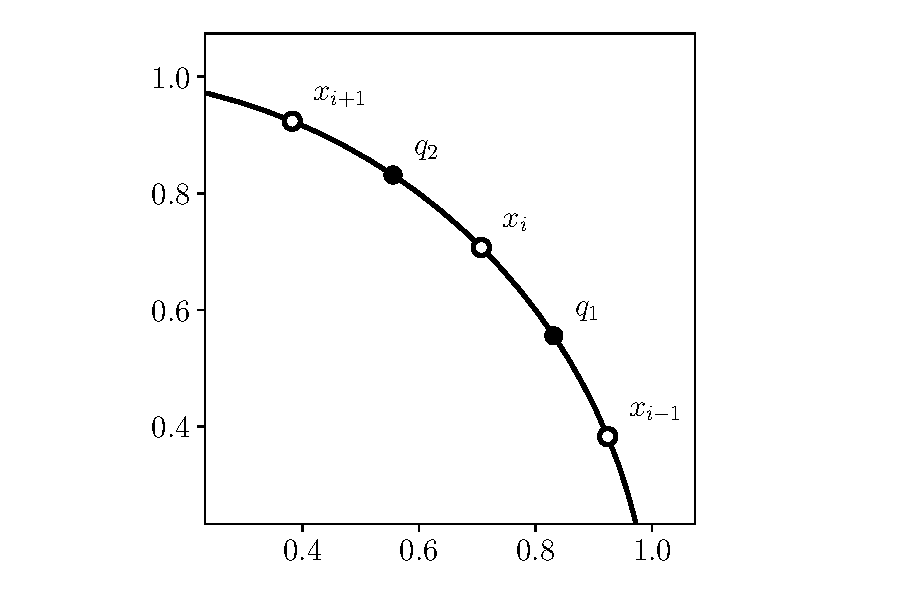
\includegraphics[width=0.8\textwidth]{figures/index.pdf}
    \caption{Bob places two points $q_1$ and $q_2$ in such a way
        on the unit circle, that they can be linearly seperated from the other
        points if and only if Alice didn't place a point at $p_i$.}
    \label{fig:index}
\end{figure}

\subsection{Sensitivity Sampling}

\subsubsection{Theoretical Foundations}

\begin{definition}[\cite{langberg-schulman-sensitivities}]
    \label{def:sensitivity}
    Let $F = \{ g_1, ..., g_n \}$ be a set of functions,
    $g_i: \mathbb{R} \rightarrow \mathbb{R}_{\geq 0}, \ i=1,...,n$ weighted by
    $w \in \mathbb{R}^n_{>0}$.
    The sensitivity of $g_i$ for $f_w(\beta) = \sum_{i=1}^n w_i g_i(\beta)$ is defined as
    \begin{equation*}
        \varsigma_i = \sup_{\beta \in \mathbb{R}^d, \ f_w(\beta) > 0} \frac{w_i g_i(\beta)}{f_w(\beta)}.
    \end{equation*}
    The total sensitivity, i.e. the sum of the sensitivities is $\mathfrak{S} = \sum_{i=1}^n \varsigma_i$.
\end{definition}

\begin{definition}[\cite{feldman-langberg-coresets}]
    A range space is a pair $\mathfrak{R} = (F, \mathcal{R})$, where F is a set
    and $\mathcal{R}$ is a family (set) of subsets of F, called
    ranges.
\end{definition}

\begin{definition}[\cite{feldman-langberg-coresets}]
    The VC-dimension $\Delta(\mathfrak{R})$ of a range space $\mathfrak{R} = (F, \mathcal{R})$ is
    the size $|G|$ of the largest subset $G \subseteq F$ such that
    \begin{equation*}
        \left| \left\{ G \cap \textup{range} \ | \ \textup{range} \in \mathcal{R} \right\} \right|
        = 2^{|G|},
    \end{equation*}
    i.e. $G$ is shattered by $\mathcal{R}$.
\end{definition}

\begin{definition}[\cite{feldman-langberg-coresets}]
    Let $F$ be a finite set of functions mapping from $\mathbb{R}^d$ to $\mathbb{R}^{\geq 0}$.
    For every $\beta \in \mathbb{R}^d$ and $r \geq 0$, let
    \begin{equation*}
        \textup{range}(F, \beta, r) = \left\{ f \in F \ | \  f(\beta) \geq r  \right\}
    \end{equation*}
    and let
    \begin{equation*}
        \mathcal{R}(F) = \left\{ \textup{range}(F, \beta, r) \ | \ \beta \in \mathbb{R}^d, \ r \geq 0  \right\}.
    \end{equation*}
    Then we call $\mathfrak{R}_F := (F, \mathcal{R}(F))$ the range space induced by F.
\end{definition}

\begin{theorem}[\cite{braverman-feldman-coresets, big-data-tiny-data}]
    Let $\mathcal{F} = \{ f_1, ..., f_n \}$ be a set of functions,
    $f_i: \mathbb{R} \rightarrow \mathbb{R}^{\geq 0}, \ i=1,...,n$ weighted by
    $w \in \mathbb{R}^n_{>0}$.
    Let $\epsilon, \delta \in (0, \frac{1}{2})$.
    Let $s_i \geq \varsigma_i$.
    Let $S = \sum_{i=1}^n s_i \geq \mathfrak{S}$.
    Given $s_i$, one can compute in time $O(|\mathcal{F}|)$ a set
    $\mathcal{R} \subseteq \mathcal{F}$ of
    \begin{equation*}
        O \left( \frac{S}{\epsilon^2} \left( \Delta \log S + \log \left( \frac{1}{\delta} \right) \right) \right)
    \end{equation*}
    weighted functions such that with probability $1 - \delta$ we have
    for all $\beta \in \mathbb{R}^d$ simultaneously
    \begin{equation*}
        \left| \sum_{f \in \mathcal{F}} w_i f_i(\beta) - \sum_{f \in \mathcal{R}} u_i f_i(\beta) \right| \leq \epsilon \sum_{f \in \mathcal{F}} w_i f_i(\beta)
    \end{equation*}
    where each element of $\mathcal{R}$ is sampled independently with probability
    $p_j = \frac{s_j}{S}$ from $\mathcal{F}$, $u_i = \frac{S w_j}{s_j |\mathcal{R}|}$
    denotes the weight of a function $f_i \in \mathcal{R}$ that corresponds to
    $f_j \in \mathcal{F}$, and where $\Delta$ is an upper bound on the
    VC-dimension of the range space $\mathfrak{R}_{\mathcal{F}^*}$ induced by
    $\mathcal{F}^*$. $\mathcal{F}^*$ is the set of functions $f_j \in \mathcal{F}$
    scaled by $\frac{S w_j}{s_j |\mathcal{R}|}$.
\end{theorem}

\subsubsection{Constructing the Coreset}
